%%%%%%%%%%%%%% STANDARD MODE


\documentclass[10pt]{beamer}

\mode<presentation>
{
 \usetheme{Boadilla}
\pagestyle{empty}

\setbeamerfont*{frametitle}{size=\normalsize,series=\bfseries}
\setbeamerfont*{block}{size=\normalsize,series=\bfseries}
%\setbeamertemplate{blocks}[rounded][shadow=true]
}

\definecolor{links}{HTML}{2A1B81}
\hypersetup{colorlinks,linkcolor=,urlcolor=links}


\usepackage[pdf]{pstricks}
\usepackage{pst-sigsys}


\definecolor{darkblue}{rgb}{0.0, 0.0, 0.40}
\setbeamercolor{title}{fg=darkblue}
\setbeamercolor{frametitle}{fg=darkblue}
\definecolor{darkgreen}{rgb}{0.0, 0.4, 0.0}

\usepackage{bbm}



\usepackage{etex}
% \usepackage{helvet}
\usepackage{amsmath, amssymb}
\usepackage{color}
\usepackage{asymptote}
\usepackage{mathrsfs}
\usepackage{dsfont}
\usepackage{makeidx}
\usepackage{multido}
\usepackage{hyperref}


\usepackage{pst-sigsys,pst-plot,pstricks-add}
%\usepackage{auto-pst-pdf}
\usepackage{pst-pdf}


\def\R{{\mathcal{R}}}
\def\I{{\mathcal{I}}}

\newcommand{\hl}[1]{\textbf{#1}}


\title[]{Introduction to Signals}
\author[\textcolor{blue}{Systems and Circuits}]{\textcolor{darkblue}{Pablo M. Olmos} (olmos@tsc.uc3m.es)\\ \textcolor{darkblue}{Emilio Parrado} (emipar@tsc.uc3m.es)}
\institute{\textcolor{white}{UC3M}}



\AtBeginSection[]
{
  \begin{frame}<beamer>{Index}
    \tableofcontents[currentsection,currentsubsection]
  \end{frame}
}






%%%%%%%%%%%%%%%%
\begin{document}

\frame{
\titlepage
\thispagestyle{empty}
\begin{center}

\includegraphics[scale=0.05]{Figures/uc3m-logo2.pdf}
\end{center}
}

\section{Basic definitions}

\frame{
%\frametitle{The physical world: representation by means of signals and systems}
\begin{itemize}
\item Signals: Functions that represent variations in physical magnitudes.
\item Information is contained in the variation with respect some independent variables.
\end{itemize}
\begin{figure}
\centering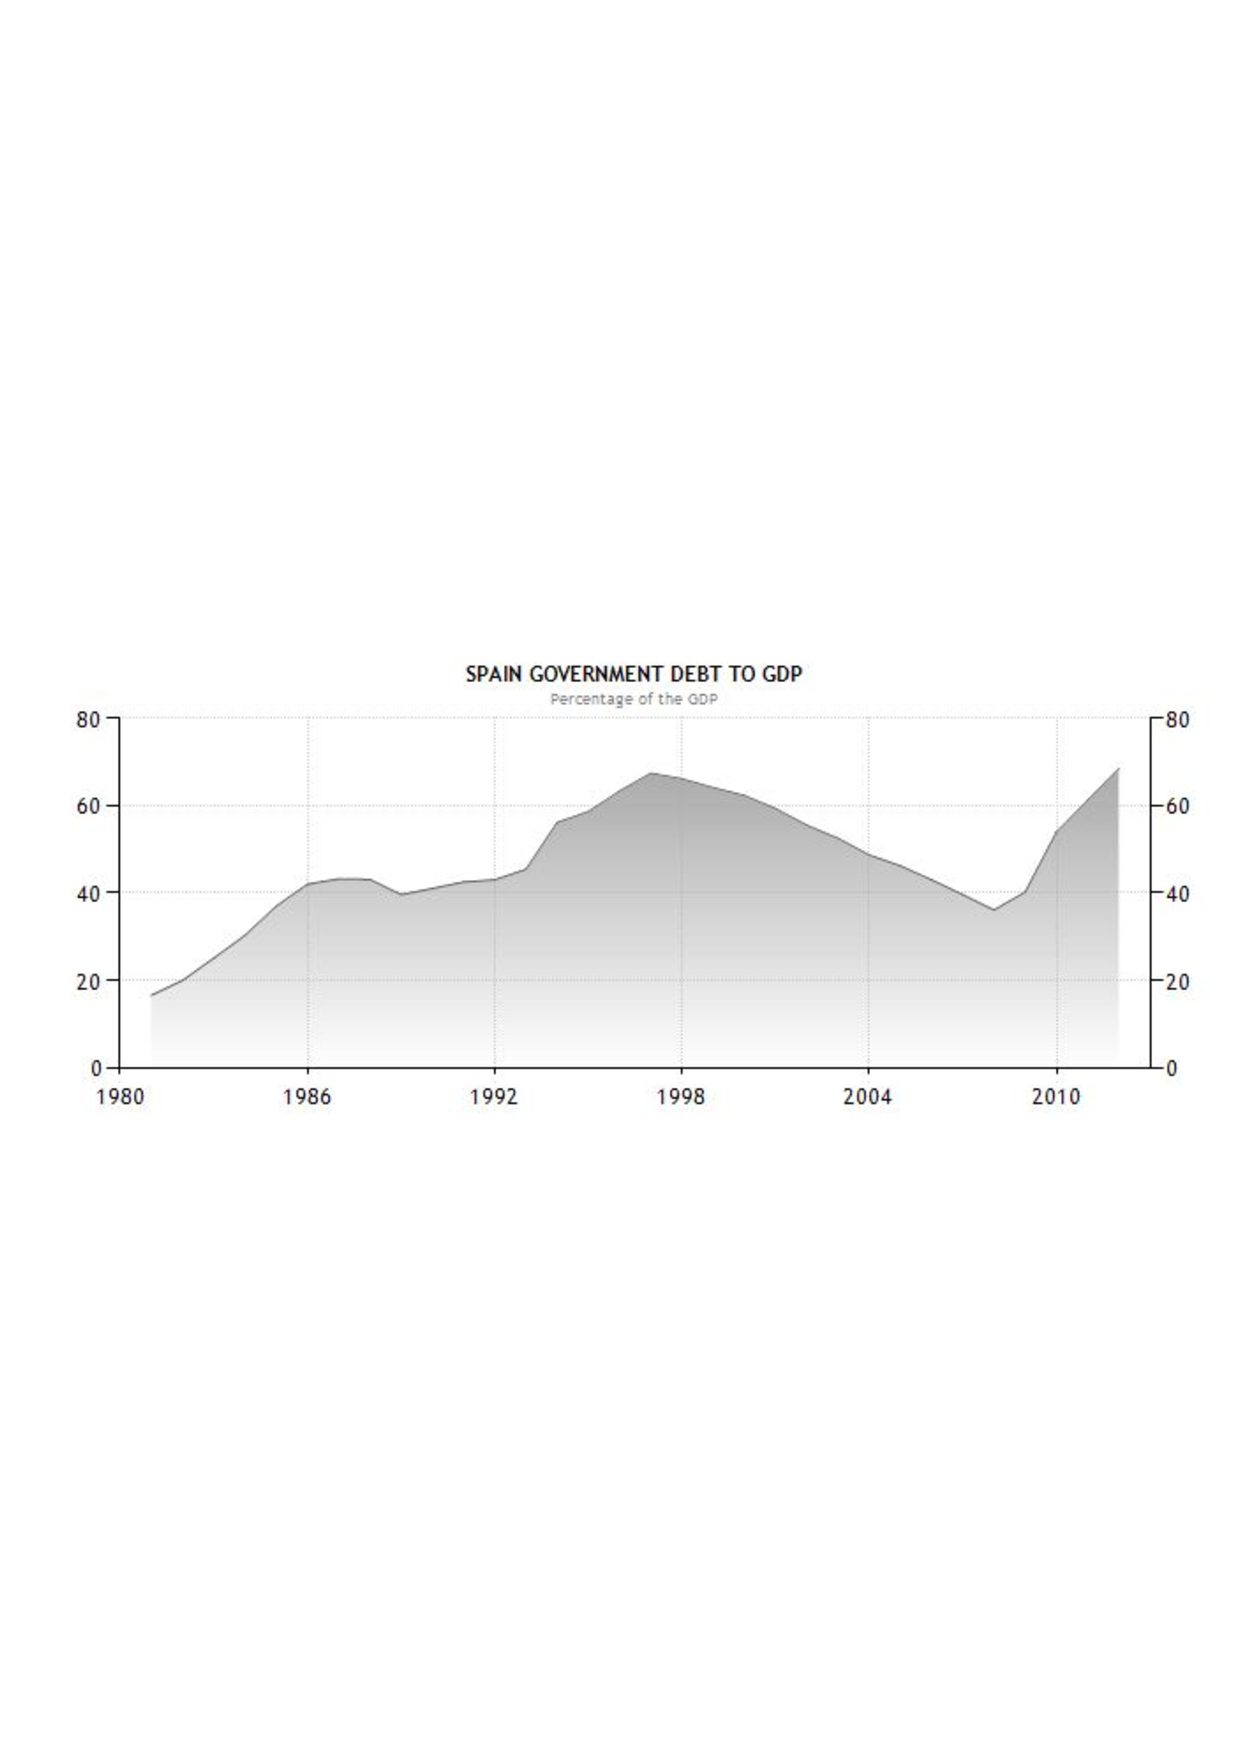
\includegraphics[scale=0.4]{Figures/Signal8.pdf}
\caption{Spanish debt evolution along the time (GDP: gross domestic product). }
\end{figure}
}

\frame{
\frametitle{Mathematically, we represent signals by functions}
\begin{itemize}
\item $x(u)$ if a \hl{one-dimensional (unidimensional)} signal with a single independent variable.
\item $\mathbf{x}(u)$ is a  \hl{$d$-dimensional  (multidimensional)} signal with a single independent variable, where
\begin{align*}
\mathbf{x}(u)=\left[
\begin{array}{c}
x_1(u) \\ x_2(u) \\ x_3(u) \\ \ldots \\ x_d(u)
\end{array}
\right]
\end{align*}
\item $x(u,t)$ is a unidimensional signal with two independent variables.
\end{itemize}
}


\frame{

\begin{block}{}
Without loss of generality, we restrict to scalar signals with a single independent variable that is referred to as \emph{time}.
\end{block}

E.g.,
\begin{itemize}
\item $T(t)$ is the temperature evolution over time.
\item $R[n]$ is the average rainfall in 20 consecutive years $n=1,\ldots,20$.
\end{itemize}


}

\frame{
\frametitle{Continuous-time signals}

\begin{block}{}
The independent variable is continuous in a given interval. Continuous-time signals are defined for a continuum of values of the independent variable.
\end{block}


\begin{itemize}
\item $x(t)$  $\forall t\in\mathbb{R}$.
\item $x(t)$  $\forall t\in[a,b]$.
\item ...
\end{itemize}


\begin{columns}
\begin{column}{0.5\textwidth}
\begin{figure}
\centering
\includegraphics[scale=0.25]{Figures/Plot1.jpg}
\caption{Vinyl record}
\end{figure}
\end{column}
\begin{column}{0.5\textwidth}
\begin{figure}
\centering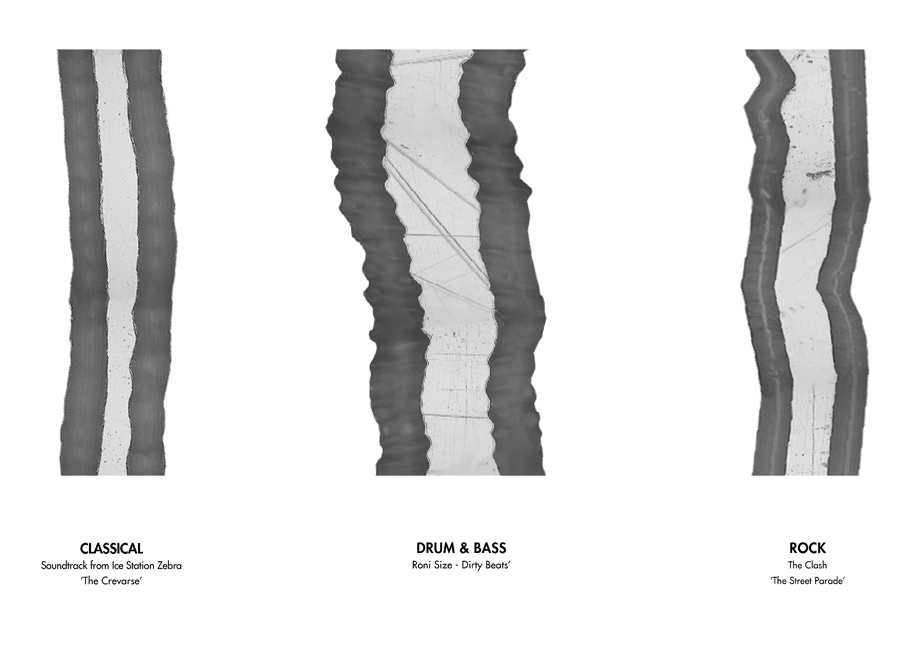
\includegraphics[scale=0.65]{Figures/Plot2.jpg}
\caption{The shape of the groove encodes the sound that will be played when the stylus goes along the groove}.
\end{figure}
\end{column}
\end{columns}

}

\frame{
\begin{figure}
\centering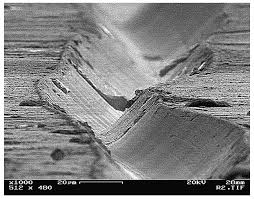
\includegraphics[scale=0.85]{Figures/Plot3.jpg}
\caption{Source. \url{http://www.synthgear.com/2014/audio-gear/record-grooves-electron-microscope}}
\end{figure}
}


\frame{
\frametitle{Discrete-time signals or sequences}

\begin{block}{}
They are only defined at discrete times, and consequently for these signals the independent variable takes on only a discrete set of values.
\end{block}

\begin{itemize}
\item $x[n]$ $\forall n\in\mathbb{Z}$.
\item $x[n]$ $\forall n\in\{-5,-4,\ldots,4,5\}$.
\item ...
\end{itemize}

\begin{alertblock}{}
They are only defined for integer values of the independent variable. Thus, \textbf{$x[1/2]$ does not exist}.
\end{alertblock}

\begin{itemize}
\item Average temperature per month in the last year $T_{\text{avg}}[n]$ $n=1,2,\ldots,12$.
\item Benefits in the stock market per day in the last year $P[n]$ $n=1,2,\ldots,365$.
\end{itemize}

}


%
%\frame{
%
%
%
%
%\begin{columns}
%\begin{column}{0.5\textwidth}
%\psset{xunit=0.5cm,yunit=0.5cm}
%\begin{center}
%\begin{pspicture}[showgrid](-2,-5)(7,4)
%  \rput(0,0){\psaxeslabels(0,0)(-2,0)(7,0){$n$}{}
%     \rput[tl](-2,6){$x[n]$}
%     \psstem[style=Stem,linecolor=red](-2,1)
%            {0,3.6,-1.7,0,3.2,-3.5,-5,0.5}}
%\end{pspicture}
%\end{center}
%\end{column}
%\begin{column}{0.2\textwidth}
%\begin{align*}
%x[-2]&=0, ~ x[-1]=3.6, ~ x[0]=-1.7\\
%x[1]&=0, ~ x[2]=3.2, ~ x[3]=-3.5\\
%x[4]&=-5, ~x[5]=0.5
%\end{align*}
%\end{column}
%\end{columns}
%
%
%}

%\frame{
%\frametitle{ Huygens probe landing on Titan (largest moon of Saturn)}
%
%\begin{exampleblock}{}
%This \textcolor{blue}{\href{http://youtu.be/fXwtDTk810s}{movie}}, built with data collected during the European Space Agency's Huygens probe on Jan. 14, 2005, shows the operation of the Descent Imager/Spectral Radiometer camera during its descent and after touchdown. 
%\end{exampleblock}
%
%Lets take a look of the signals the probe was transmitting to Earth (about 1 355 357 880 km away).
%
%\begin{figure}
%\begin{tabular}{cc}
%\centering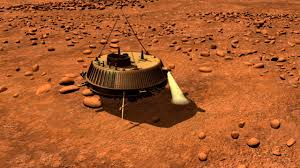
\includegraphics[scale=0.5]{Figures/probe.jpg} & \centering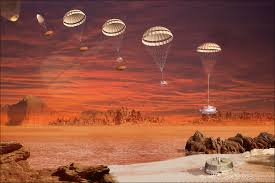
\includegraphics[scale=0.47]{Figures/titan_1.jpg}
%\end{tabular}
%\end{figure}
%
%}
%

\frame{
\frametitle{Complex and real signals}

\begin{block}{}
$x(t)$ and $x[n]$ are \hl{real signals} if  $x(t)\in\mathbb{R}$ $\forall t$ and $x[n]\in\mathbb{R}$ $\forall n$. 
\end{block}
E.g. for $\alpha,\beta\in\mathbb{R}$, the following signals are real
\begin{align*}
x(t)&=\text{e}^{-\alpha t}+\beta t \\
x(t)&= \cos(2\pi t) t^2 +3\\
x[n]&= \alpha^{|n|}\\
x[n]&= \sum_{u=-\infty}^{n} \alpha^{|n|}
\end{align*}



%\item $x(t)$ and $x[n]$ are \hl{complex signals} if  $x(t)\in\mathbb{C}$ $\forall t$ and $x[n]\in\mathbb{C}$ $\forall n$

\begin{alertblock}{}
Real signals are a part of the \emph{physical world}, physical magnitudes are naturally represented by real signals.
\end{alertblock}

}





\frame{
\frametitle{Complex and real signals}

\begin{block}{}
$x(t)$ and $x[n]$ are \hl{complex signals} if  $x(t)\in\mathbb{C}$ $\forall t$ and $x[n]\in\mathbb{C}$ $\forall n$.
\end{block}
E.g. for $\alpha,\beta\in\mathbb{C}$, the following signals are complex
\begin{align*}
x(t)&=\text{e}^{-\alpha t}+\beta t,\\
x(t)&= \cos(2\pi t) t^2 +3 t j\\
x[n]&=\frac{4n+j8n}{n^2+j4\pi n}\\
x[n]&= \sum_{u=-\infty}^{n} (-1)^{u/2}\alpha^{|n|}
\end{align*}

}

\frame{
\frametitle{Complex and real signals}

\begin{itemize}
\item Complex numbers and, by extension, complex signals have no physical existence.
\item A huge list of real-life physical effects, though they're described by real numbers, are nevertheless best understood through the mathematics of complex numbers. 
\item Often, decomposing a real signal in terms of operations between complex signals is very valuable for transforming the problem into a much simpler problem.
\end{itemize}



\begin{exampleblock}{}
\begin{itemize}
\item Review of complex numbers!
\end{itemize}
\end{exampleblock}

}

\frame{
\frametitle{We need complex signals to understand the electromagnetic spectrum!}

\begin{figure}
\centering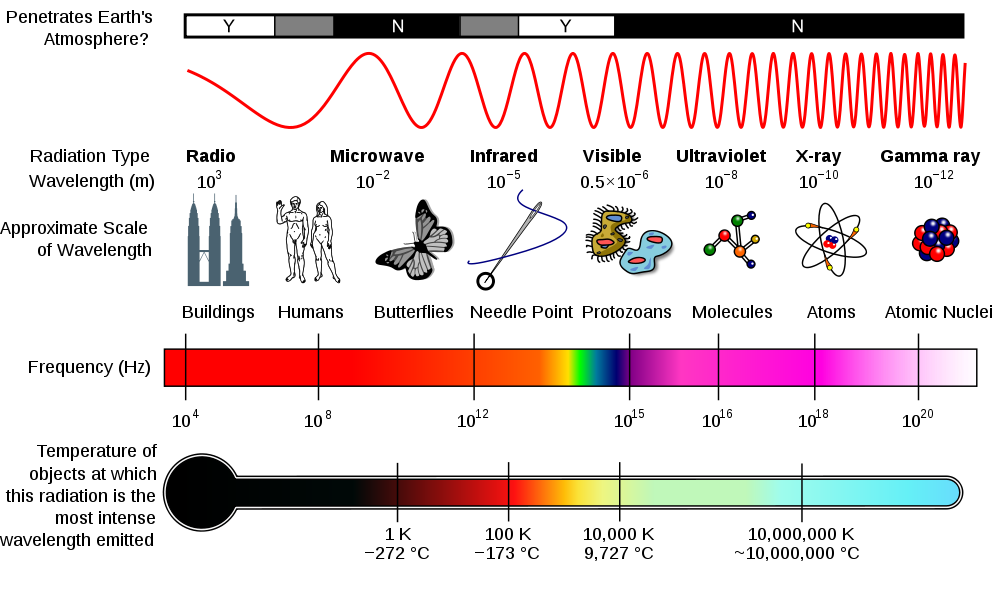
\includegraphics[scale=0.25]{Figures/Plot4.png}
\caption{Source. \url{http://earthsky.org/space/what-is-the-electromagnetic-spectrum}}
\end{figure}

}

%\frame{
%
%\begin{exampleblock}{}
%Let $a$ and $b$  be real quantities, using the \emph{Euler formula} for any real quantity $\alpha$ the following holds
%\begin{align*}
%a\cos(\alpha)-b\sin(\alpha)=\Re\left[(a+jb)\text{e}^{j\alpha}\right]
%\end{align*}
%\end{exampleblock}
%
%
%}





\frame{

\begin{alertblock}{}
Complex signals are widely used in signal processing.  You can think of a given complex signal $x(t)$ as $2$-dimensional signal
\begin{align*}
\left[
\begin{array}{c}
x_{\R}(t) \\ x_{\I}(t)
\end{array}
\right],
\qquad
\left[
\begin{array}{c}
|x|(t) \\ \angle(x(t))
\end{array}
\right]=
\left[
\begin{array}{c}
\sqrt{x_{\R}^2(t)+x_{\I}^2(t)} \\ \displaystyle \arctan({\frac{x_{\I}(t)}{x_{\R}(t)}})
\end{array}
\right]
\end{align*}
\end{alertblock}




}


\section{Operations with signals}

\frame{
\frametitle{Operations with signals	}

\begin{itemize}
\item Standard operations with mathematical functions.
\item They are performed pointwise.
\end{itemize}

\begin{block}{}
Given $x[n]$ and $y[n]$, $z[n]=x[n]+y[n]$ at $n=3$ is $x[3]+y[3]$.
\end{block}
}

\frame{
\frametitle{Sum of two signals}
Compute the sum between the following two signals:

\begin{figure}
\centering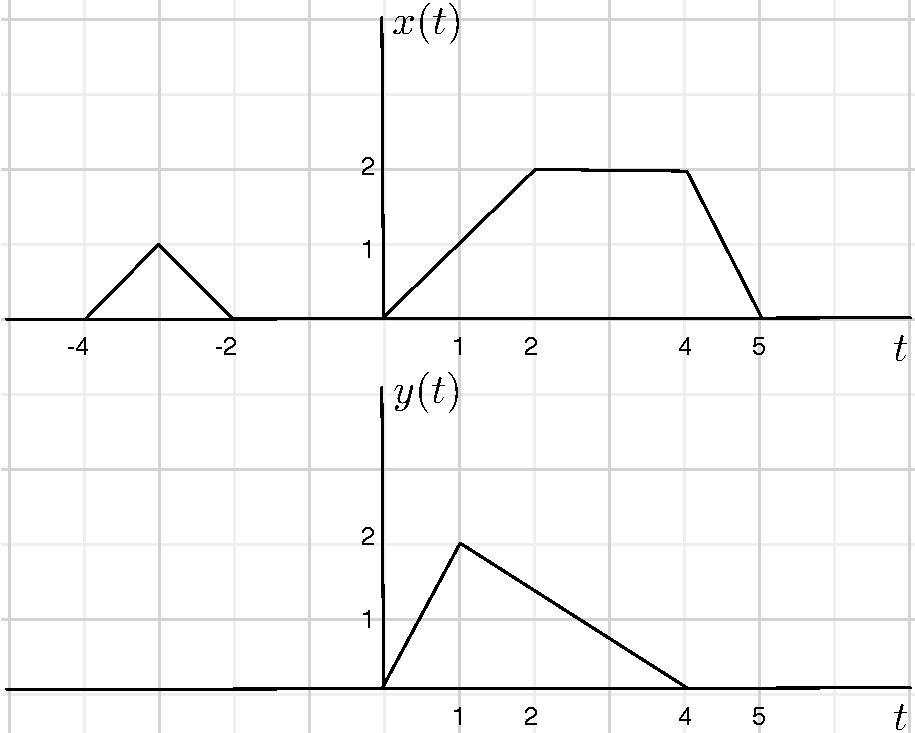
\includegraphics[scale=0.5]{Figures/sum.pdf}
\end{figure}

}

\frame{
Sol.

\begin{figure}
\centering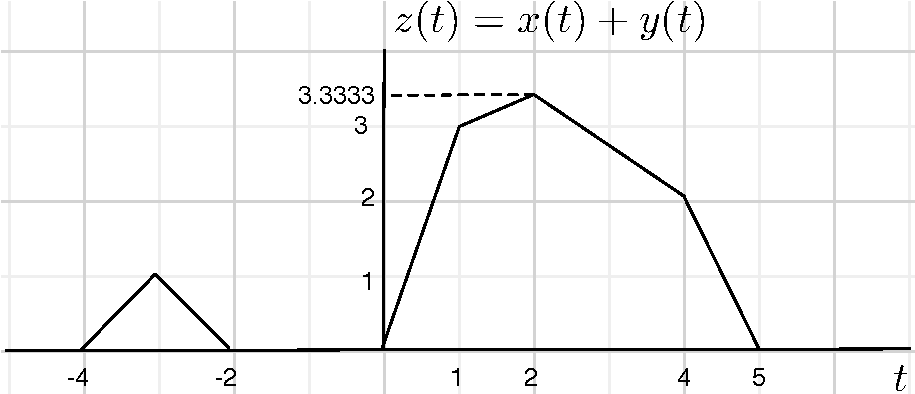
\includegraphics[scale=0.5]{Figures/sum_sol.pdf}
\end{figure}



}

\frame{
\frametitle{Product of two signals}
\begin{block}{}
Given 
\begin{align*}
x(t)&=2t^2,\qquad y(t)=t
\end{align*}
then 
\begin{align*}
z(t)= x(t) \times y(t)=2t^3
\end{align*}
\end{block}

\begin{block}{}
Given
\begin{align*}
x[n]=(3n+4jn^2)\qquad y[n]=(0.5)^n+2jn
\end{align*}
then
\begin{align*}
z[n]=3n(0.5)^n-8n^3+6jn^2+4jn^2(0.5)^n
\end{align*}
\end{block}

}


\frame{
\frametitle{Absolute value or modulus}
\begin{itemize}
\item Given $x(t)$ 
\begin{align*}
|x(t)|=\sqrt{x_{\R}^2(t)+x_{\I}^2(t)} 
\end{align*}
\item If $x(t)$ is a real signal, then
\begin{align*}
|x(t)|=\left\{
\begin{array}{cc}
x(t) & x(t)\geq 0\\
-x(t) & x(t)< 0
\end{array}
\right.
\end{align*}
\end{itemize}


}


\frame{
Other operations that you already know how to compute. Given $x(t)=\text{e}^{-4t}+3j\cos(2\pi t)$, compute
\begin{align*}
y(t)&=\frac{\partial x(t)}{\partial t}\\
y(t)&=\int_{-5}^{t}x(\tau)d\tau\\
y(t)&=\angle x(t)=\arctan({\frac{x_{\I}(t)}{x_{\R}(t)}})\\
&....
\end{align*}


}


\section{Transforming the independent variable}


\frame{

\begin{block}{}
In many situations it is important to consider signals related by a modification of the \hl{independent variable} (time).
\end{block}

Given $x(t)$ or $x[n]$, 

\begin{itemize}
\item $y[n]=x[-n]$
\item $g(t)=x(t+2)$
\item $z[n]=x[2n]$
\item $w(t)=x(-t/3+4)$
\item ....
\end{itemize}


}


\frame{
\frametitle{Time shift}
\begin{block}{}
Given $x(t)$, 
\begin{align}\nonumber
y(t)=x(t)\Big|_{t'=t-t_0}=x(t-t_0)
\end{align}
is a shifted version of $x(t)$.
\end{block}
\begin{block}{}
Given $x[n]$, 
\begin{align}\nonumber
y[n]=x[n]\Big|_{n'=n-n_0}=x[n-n_0]
\end{align}
is a shifted version of $x[n]$.
\end{block}
}

\frame{
\frametitle{Example (Problem 1.a)}

\begin{figure}
\centering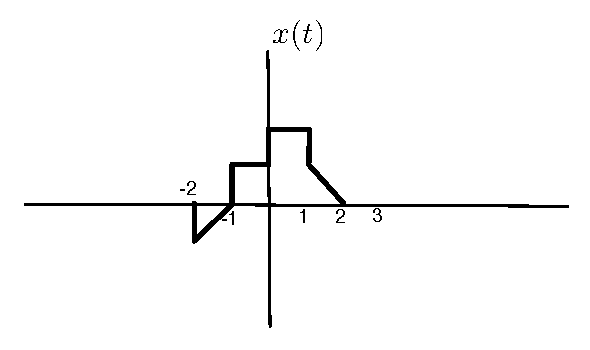
\includegraphics[scale=0.7]{Figures/Signal_1.pdf}
\end{figure}

Plot the following signals
\begin{itemize}
\item $y(t)=x(t-1)$
\item $y(t)=x(t+3)$
\end{itemize}
}

\frame{
Sol.
\begin{figure}
\centering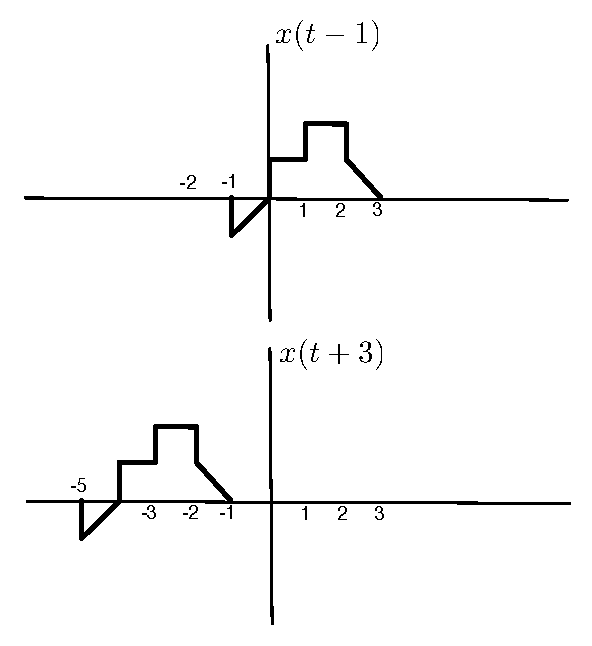
\includegraphics[scale=0.7]{Figures/Signal_2.pdf}
\end{figure}
}

\frame{
\frametitle{Temporal Inversion}
\begin{block}{}
Given $x(t)$, 
\begin{align}\nonumber
y(t)=x(-t)
\end{align}
is the temporal inversion of $x(t)$.
\end{block}

\begin{block}{}
Given $x[n]$, 
\begin{align}\nonumber
y[n]=x[-n]
\end{align}
is the temporal inversion of  $x[n]$. 
\end{block}

}

\frame{
\frametitle{Example}

\begin{figure}
\centering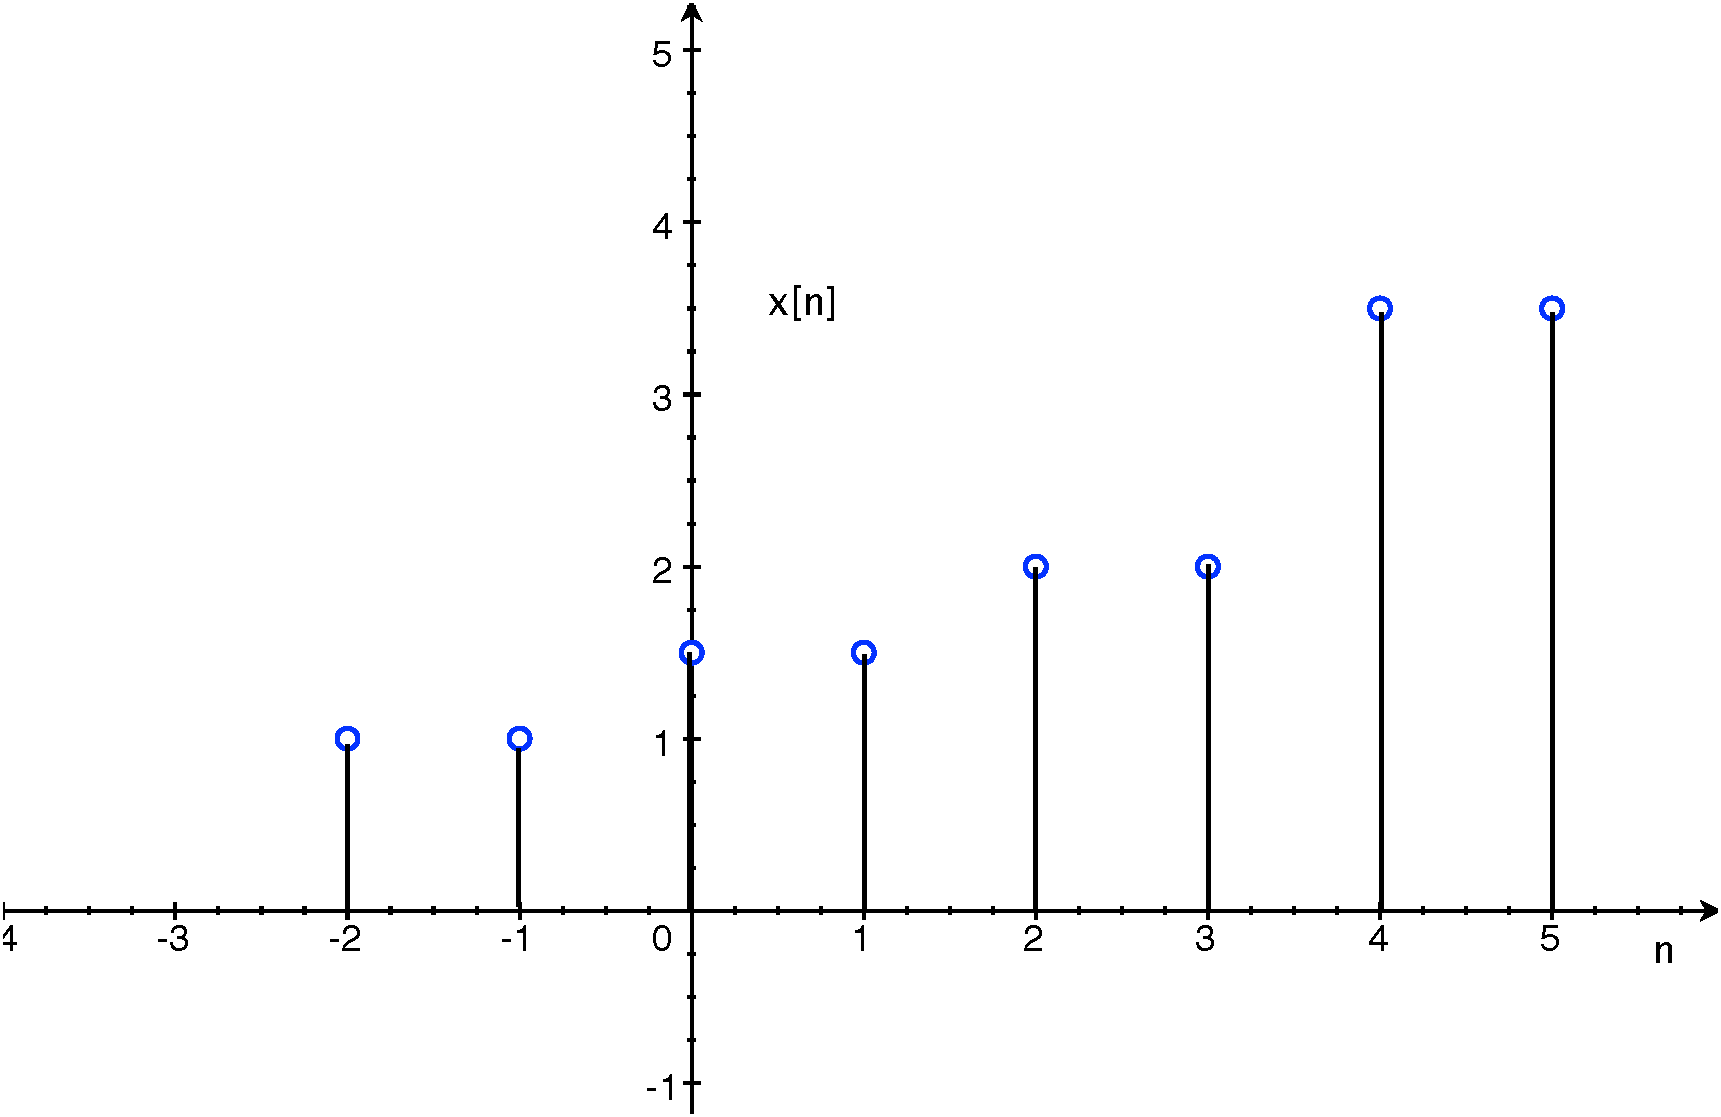
\includegraphics[scale=0.2]{Figures/Abatida.pdf}
\end{figure}

Plot the following signal
\begin{itemize}
\item $y[n]=x[-n]$
\end{itemize}
}

\frame{
Sol.
\begin{figure}
\centering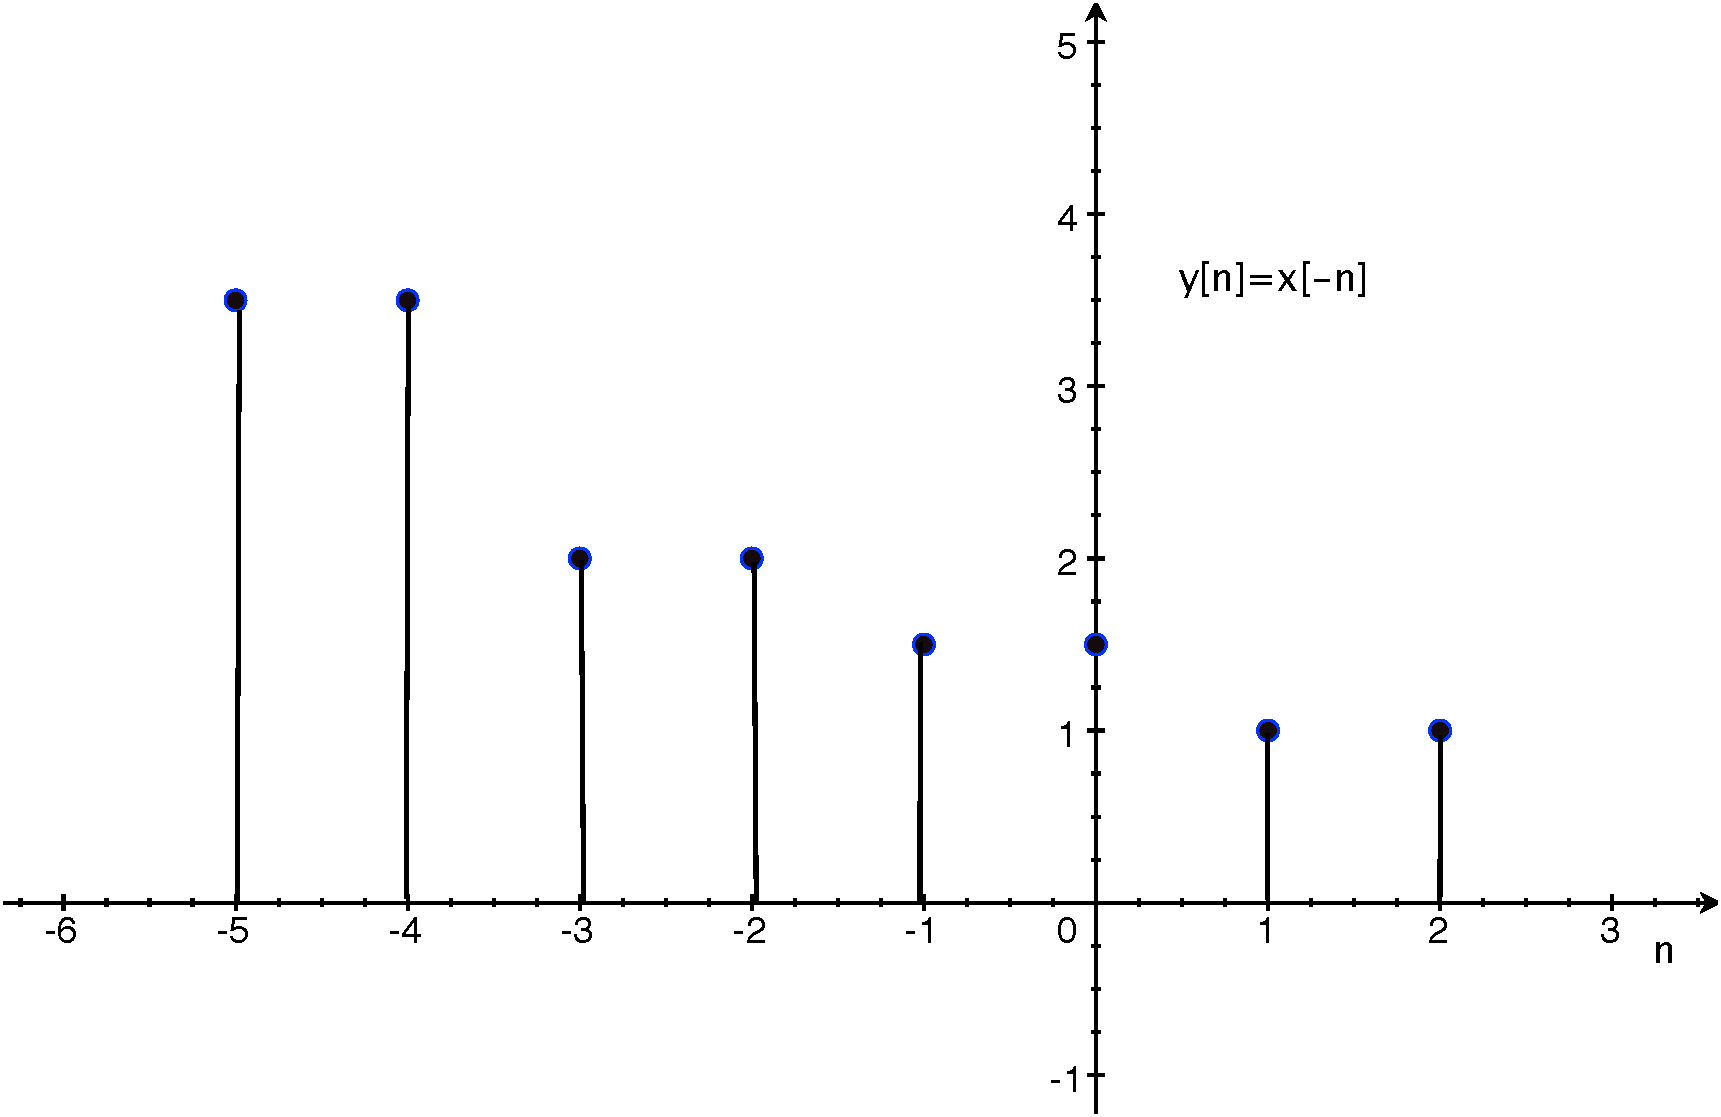
\includegraphics[scale=0.2]{Figures/Abatida2.pdf}
\end{figure}
}




\frame{
\frametitle{Time scale of a continuous-time signal}

\begin{block}{}
Given $x(t)$, 
%\begin{align}\nonumber
%y(t)=x(t)\Big|_{t'=\alpha t}=x(\alpha t)
%\end{align}
\begin{align}\nonumber
y(t)=x(\alpha t)
\end{align}
is a scaled version of $x(t)$.
\end{block}

\begin{block}{}
Given $x[n]$, 
%\begin{align}\nonumber
%y[n]=x[n]\Big|_{n'=\alpha n}=x[\alpha n]
%\end{align}
\begin{align}\nonumber
y[n]=x[\alpha n]
\end{align}
is a scaled version of $x[n]$. 
\end{block}


\begin{block}{}
\begin{itemize}
\item If $|\alpha | < 1$ the signal is \hl{expanded} 
\item If $|\alpha | > 1$ the signal is \hl{contracted}
\end{itemize}
\end{block}

}

\frame{
\frametitle{Example (Problem 1.e)}

\begin{figure}
\centering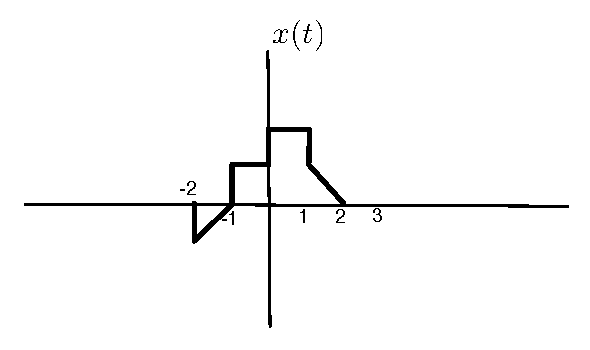
\includegraphics[scale=0.7]{Figures/Signal_1.pdf}
\end{figure}

Plot the following signals
\begin{itemize}
\item $y_1(t)=x(t/3)$
\item $y_2(t)=x(2t)$
\item $z_1(t)=y_1(3t)$
\item $z_2(t)=y_2(t/2)$
\item $y_3(t)=x(-t)$
\end{itemize}
}

\frame{
Sol.

\begin{columns}[T]
\begin{column}{0.5\textwidth}
\centering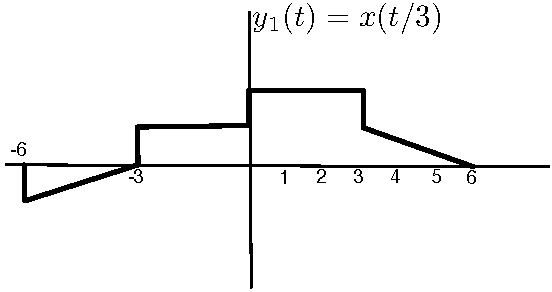
\includegraphics[scale=0.6]{Figures/Signal_3.pdf}
\end{column}
\begin{column}{0.5\textwidth}
\centering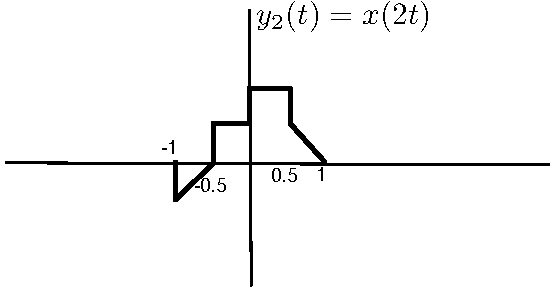
\includegraphics[scale=0.6]{Figures/Signal_4.pdf}
\end{column}
\end{columns}

\begin{align*}
z_1(t)&=y_1(3t) ~~\overset{y_1(t)=x(t/3)}{\Rightarrow} ~~ z_1(t)=x(t)\\\\
z_2(t)&=y_2(t/2) ~~\overset{y_2(t)=x(2t)}{\Rightarrow} ~~ z_2(t)=x(t)
\end{align*}

\begin{block}{}
Time scaling of a continuous-time signal is a \hl{reversible operation}.
\end{block}
}

\frame{

\begin{figure}
\centering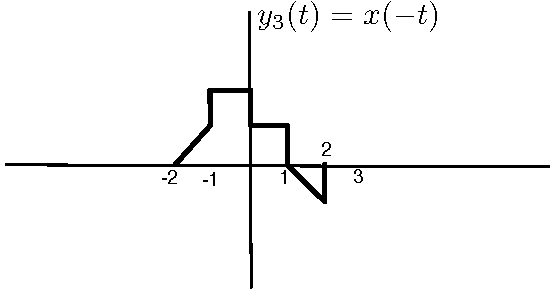
\includegraphics[scale=0.7]{Figures/Signal_22.pdf}
\end{figure}

}



\frame{
\frametitle{Scaling a discrete-time signal}

Given $x[n]$ ~$n\in\mathbb{Z}$, 
\begin{block}{}
\begin{itemize}
\item $y[n]=x[2n]$ is well defined for any integer $n$. 
\item $y[n]$ is called \textbf{a compressed version} of $x[n]$.
\item We throw away samples of $x[n]$, \hl{compressing is NOT a reversible operation}.
\end{itemize}
\end{block}

\begin{exampleblock}{}
\begin{itemize}
\item $z[n]=x[n/2]$ is NOT defined for $n$ odd. 
\item We just assume $z[n]$ at $n$ odd is $0$.
\item We don't throw away samples of $x[n]$, \hl{it is a reversible operation}.
\end{itemize}
\end{exampleblock}

}


\frame{
\frametitle{Example }

\begin{figure}
\centering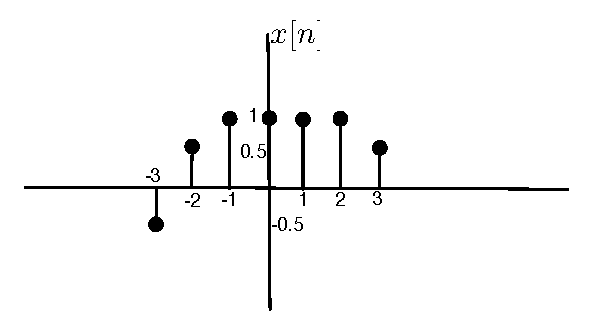
\includegraphics[scale=0.7]{Figures/Signal_5.pdf}
\end{figure}

Plot the following signals
\begin{itemize}
\item $y_1[n]=x[3n]$
\item $y_2[n]=x[n/3]$
\end{itemize}
}

\frame{
Sol.

\begin{columns}[T]
\begin{column}{0.3\textwidth}
\centering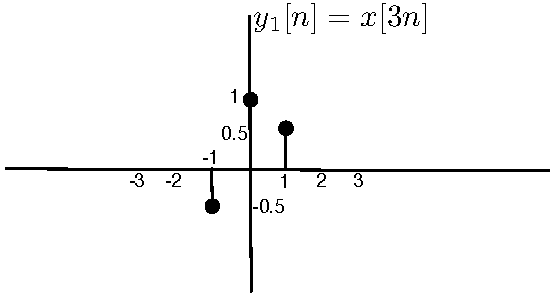
\includegraphics[scale=0.6]{Figures/Signal_6.pdf}
\end{column}
\begin{column}{0.7\textwidth}
\centering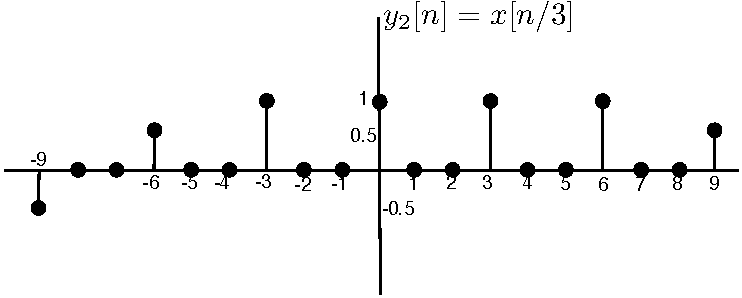
\includegraphics[scale=0.6]{Figures/Signal_7.pdf}
\end{column}
\end{columns}
}

\frame{
\frametitle{Shifting a scaled signal}
Given $y(t)=x(\alpha t)$, if we shift $y(t)$ a time $t_0$ we get
\begin{align}\nonumber
z(t)=y(t-t_0) ~~\overset{y(t)=x(\alpha t)}{\Rightarrow} ~~z(t)=x(\alpha t-\alpha t_0).
%y(t)\Big|_{t'=t-t_0}=x(\alpha t)\Big|_{t'=t-t_0}=x(\alpha t-\alpha t_0).
\end{align}

\begin{columns}[T]
\begin{column}{0.25\textwidth}
\centering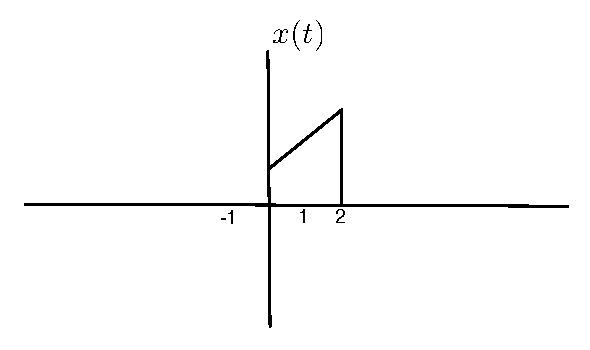
\includegraphics[scale=0.4]{Figures/Signal_8.pdf}
\end{column}
\begin{column}{0.25\textwidth}
\centering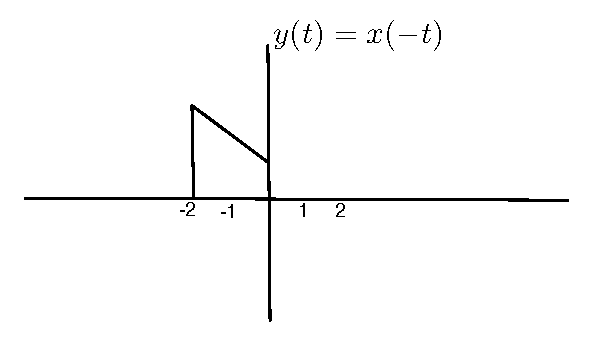
\includegraphics[scale=0.4]{Figures/Signal_9.pdf}
\end{column}
\begin{column}{0.5\textwidth}
\centering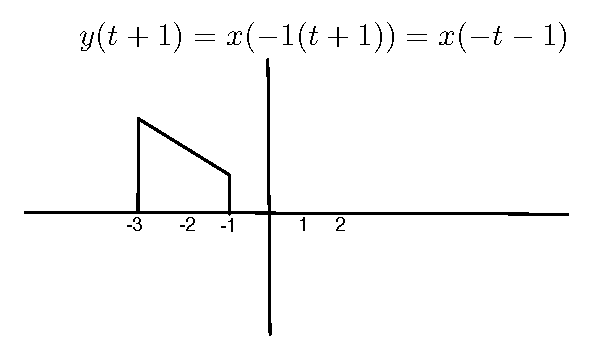
\includegraphics[scale=0.4]{Figures/Signal_10.pdf}
\end{column}
\end{columns}

\begin{alertblock}{}
Thus given $y(t)=x(\alpha t)$, $y(t-t_0)$ \textbf{is NOT equal to} $x(\alpha t-t_0)$.
\end{alertblock}
\begin{exampleblock}{Scaling a shifted signal}
Given $z(t)=x(t-t_0)$, then $z(\alpha t)=x(\alpha t-t_0)$.
\end{exampleblock}

}

\frame{
\frametitle{Time shift and time scaling. \textbf{Continuous-time signals}}
Given $x(t)$, plot
\begin{align}\nonumber
y(t)=x(\alpha t+b)
\end{align}
We have two equivalent alternatives:

\begin{block}{\textbf{Method-1}: First shift, then scale }
\begin{enumerate}
\item $z(t)=x(t+b)$.
%\item $y(t)=z(t)\Big|_{t'=\alpha t}=x(\alpha t+b)$.
\item $y(t)=z(\alpha t) ~~\overset{z(t)=x(t+b)}{\Rightarrow} ~~  y(t)=x(\alpha t+b)$.
\end{enumerate}
\end{block}

\begin{exampleblock}{\textbf{Method-2}: First scale, then shift}
\begin{enumerate}
\item $z(t)=x(\alpha t)$
%\item $y(t)=z(t)\Big|_{t'=t+\mathbf{\color{red}{b/\alpha}}}=x(\alpha t)\Big|_{t'=t+\mathbf{\color{red}{b/\alpha}}}=x(\alpha(t+b/\alpha))=x(\alpha t+b)$.
\item $y(t)=z(t+\mathbf{\color{red}{b/\alpha}})~~\overset{z(t)=x(\alpha t)}{\Rightarrow} ~~ y(t)=x(\alpha t+b)$.
\end{enumerate}
\end{exampleblock}

}

\frame{
\textbf{Method-1}
\frametitle{Examples from the collection of problems (Problem 1.d)}
\begin{columns}[T]
\begin{column}{0.3\textwidth}
\centering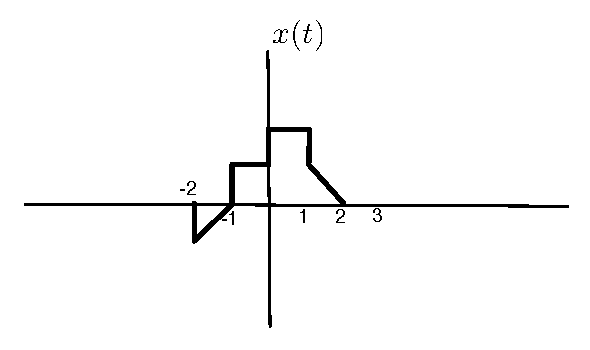
\includegraphics[scale=0.6]{Figures/Signal_1.pdf}
\end{column}
\begin{column}{0.7\textwidth}
\centering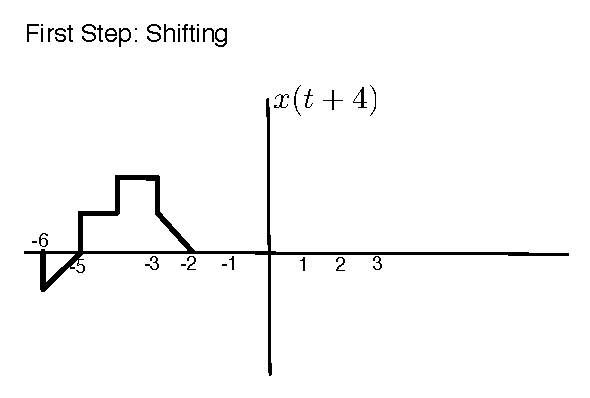
\includegraphics[scale=0.6]{Figures/Signal_11.pdf}
\end{column}
\end{columns}
\centering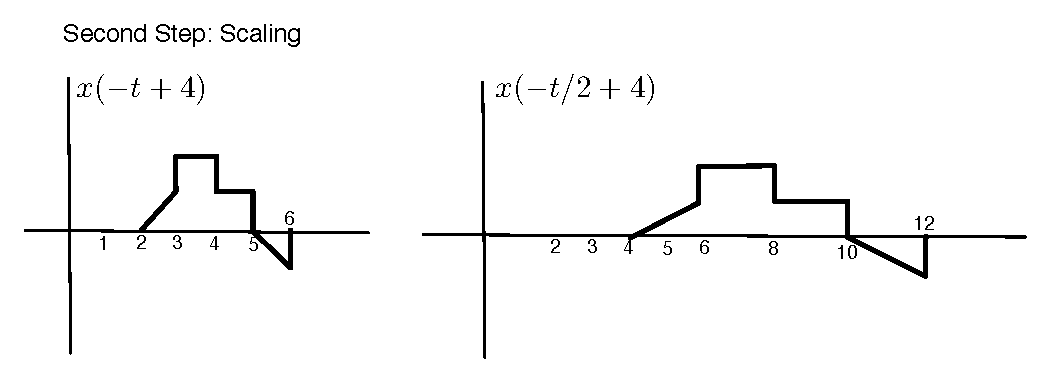
\includegraphics[scale=0.6]{Figures/Signal_12.pdf}
}

\frame{
\textbf{Method-2}
\begin{figure}
\centering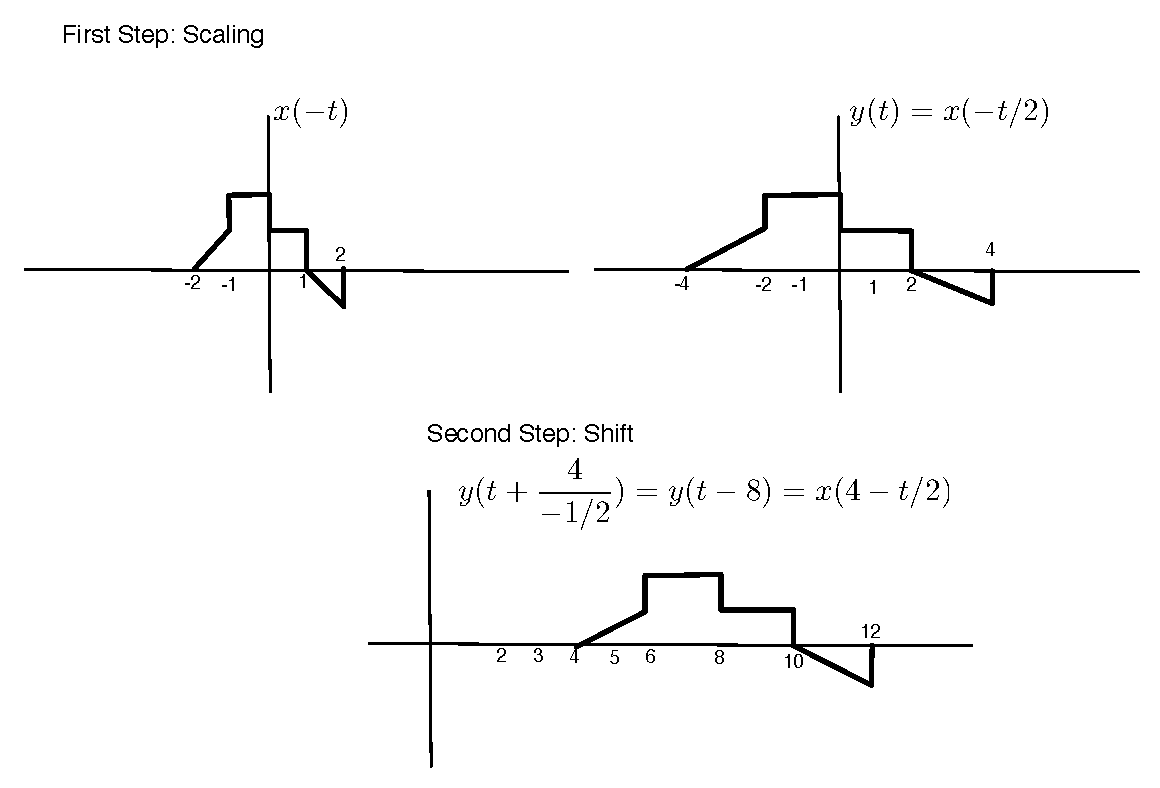
\includegraphics[scale=0.6]{Figures/Signal_18.pdf}
\end{figure}
}

\frame{
\frametitle{Time shift and time scaling. \textbf{Discrete-time signals}}
Given $x[n]$, plot
\begin{align}\nonumber
y[n]=x[\alpha n+b],
\end{align}
where $b$ is an integer. 

\begin{block}{First shift, then scale}
\begin{enumerate}
\item $z[n]=x[n+b]$.
\item $y[n]=z[\alpha n] ~~\overset{z[n]=x[n+b]}{\Rightarrow} ~~ y[n]=x[\alpha n+b]$.
\end{enumerate}
\end{block}

}


\frame{
\frametitle{Example}
\begin{columns}[T]
\begin{column}{0.3\textwidth}
\centering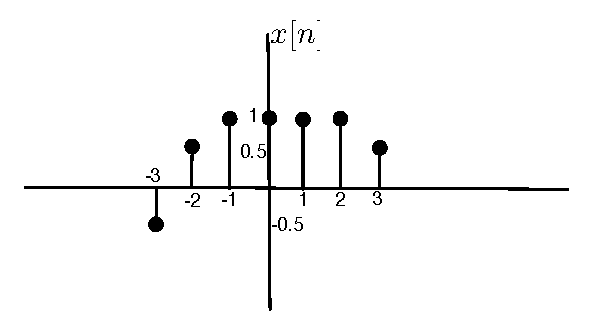
\includegraphics[scale=0.6]{Figures/Signal_5.pdf}
\end{column}
\begin{column}{0.7\textwidth}
\centering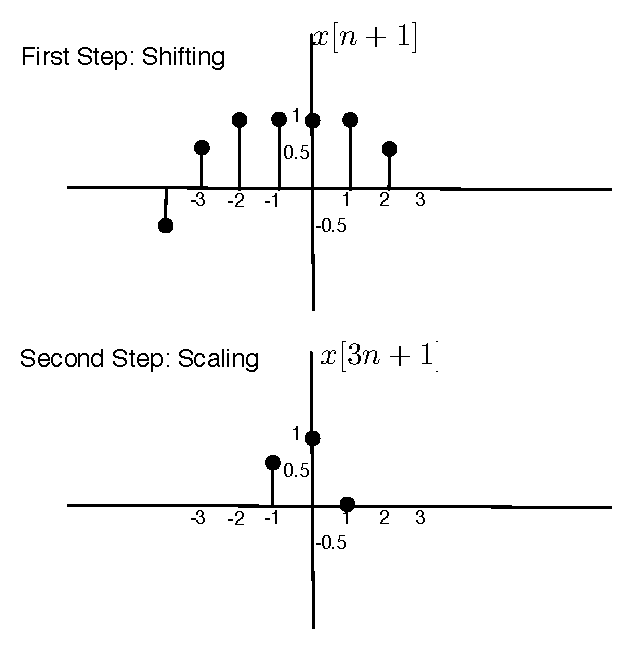
\includegraphics[scale=0.6]{Figures/Signal_13.pdf}
\end{column}
\end{columns}

}

\frame{
\begin{alertblock}{}
Caution!! In general, doing first the scaling and then shifting the sequence is not possible.
\end{alertblock}

E.g., $y[n]=x[3n+1]$
\begin{itemize}
\item Scaling: $z[n]=x[3n]$.
\item Shifting: $w[n]=z[n+1/3]!!$ Not possible! The minimum shift is 1.
\end{itemize}

}




\frame{
\frametitle{Problem 5}
Given $y(t)$,
\begin{figure}
\centering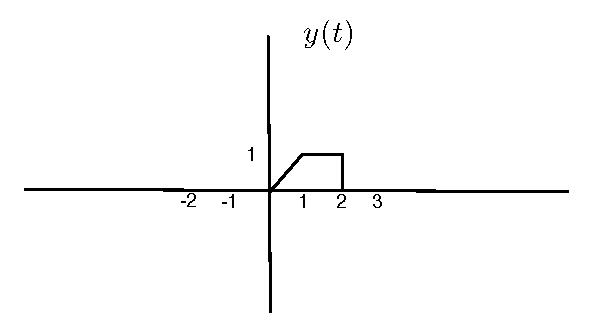
\includegraphics[scale=0.6]{Figures/Signal_14.pdf}
\end{figure}

We know that $y(t)=0.2x(-2t-3)$. Plot $x(t)$.
\begin{exampleblock}{}
Lets solve the problem following two ways.
\end{exampleblock}
}

\frame{
\textbf{Method-1}\\

\frametitle{Example 2}
\textbf{Step-1:} Lets compute $z(t)=y(-t/2)=0.2x(-2(-t/2)-3)=0.2x(t-3)$.
\begin{figure}
\centering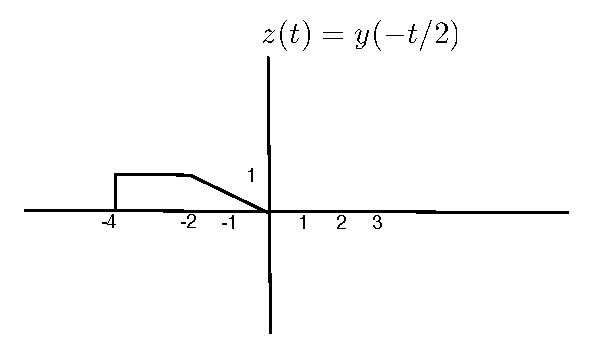
\includegraphics[scale=0.6]{Figures/Signal_15.pdf}
\end{figure}
}

\frame{
\textbf{Method-1}\\

\frametitle{Example 2}
\textbf{Step-2:} Lets compute $5z(t+3)=x((t+3)-3)=x(t)$.
\begin{figure}
\centering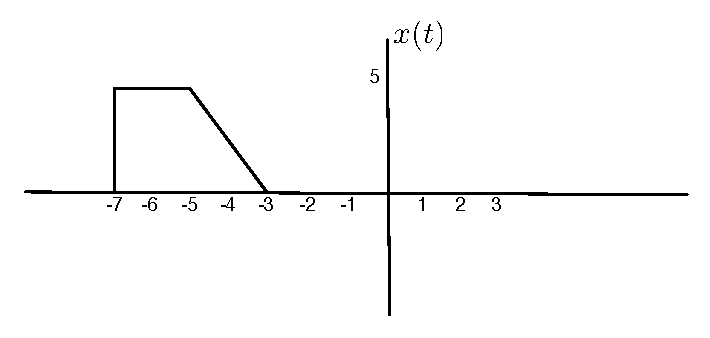
\includegraphics[scale=0.6]{Figures/Signal_16.pdf}
\end{figure}

\begin{exampleblock}{}
To check the solution, compute $w(t)=0.2x(t-3)$ and then check that $y(t)=w(-2t)$.
\end{exampleblock}
}

\frame{
\textbf{Method-2}\\

\frametitle{Example 2}
\textbf{Step-1:} Lets compute $z(t)=y(t-\frac{3}{2})=0.2x(-2(t-\frac{3}{2})-3)=0.2x(-2t+3-3)=0.2x(-2t)$.
\begin{figure}
\centering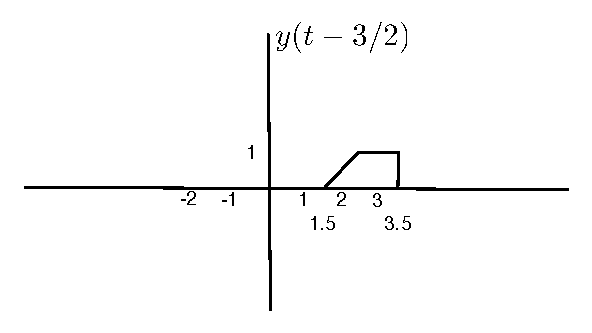
\includegraphics[scale=0.6]{Figures/Signal_19.pdf}
\end{figure}
}

\frame{
\textbf{Method-2}\\

\frametitle{Example 2}
\textbf{Step-2:} Lets compute $5y(-1/2t)=x(t)$.
\begin{figure}
\centering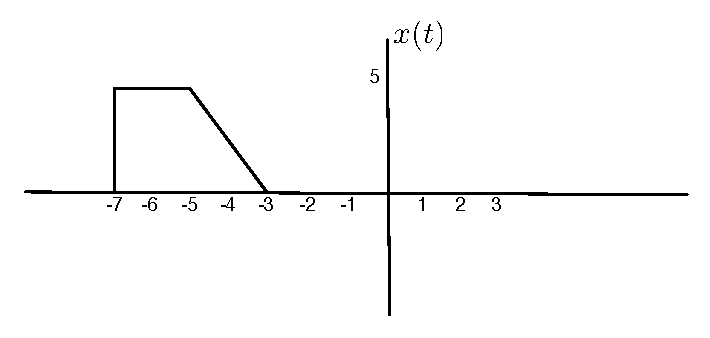
\includegraphics[scale=0.6]{Figures/Signal_16.pdf}
\end{figure}

\begin{exampleblock}{}
To check the solution, compute $w(t)=x(-2t)$ and then check that $y(t)=w(t+\frac{-3}{-2})=w(t+\frac{3}{2})=x(t)$.
\end{exampleblock}
}



\frame{
\frametitle{Example 3 (You should do it at home)}
The four signals are just combinations of (scaled) versions of the following ones:
\begin{figure}
\centering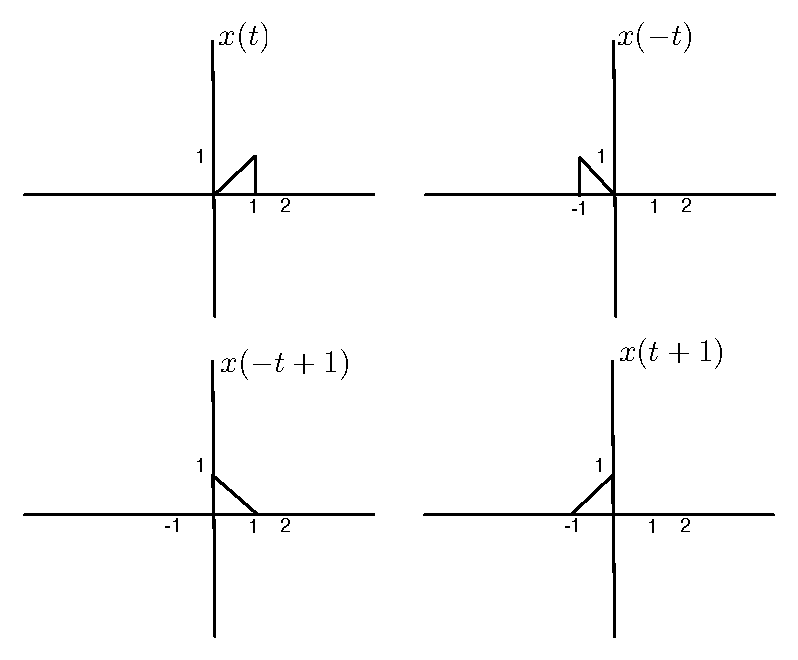
\includegraphics[scale=0.6]{Figures/Signal_17.pdf}
\end{figure}
}

\end{document}
